% !TEX root = ../my_thesis.tex

\section{Ergebnisse}
Im vorliegenden Kapitel werden die Ergebnisse der durchgeführten Experimente präsentiert. In dieser Arbeit gibt ein Evaluationsergebnis eines Netzwerkes die Abweichung der Position in Metern sowie Orientierung in Grad an und der Median der Evaluationsergebnisse bestimmt die Akkuratesse eines Netzwerkes. Somit bildet sich die Akkuratesse eines Netzwerkes aus der Zusammensetzung von Positions-  sowie Orientierungsfehler. Sowohl ein Evaluationsergebnis als auch eine Akkuratesse ist gegenüber Seinesgleichen besser genau dann, wenn deren Positionsfehler kleiner ist.

Im weiteren Verlauf dieses Kapitels werden zuerst die Reproduktionsergebnisse von BIM-PoseNet \cite{acharyaBIMPoseNetIndoorCamera2019} angegeben. Anschließend werden die Evaluationsergebnisse der trainierten Netzwerke angezeigt.

\subsection{Reproduktion der Ergebnisse von BIM-PoseNet}
Die Ergebnisse der Experimente von \citet{acharyaBIMPoseNetIndoorCamera2019}, die das PoseNet Model mit Gradientenbilder der karikaturistischen Daten sowie synthetischen Kantenbilder trainierten und anschließend mit den Gradientenbilder der realen Daten evaluierten, konnten näherungsweise (vgl. Tabelle \ref{tab:reproduction}) reproduziert werden. Der Trainingsprozess wurde je Datensatztyp 5-mal wiederholt und die bessere Akkuratesse wurde behalten. Eine exakte oder bessere Reproduktion der Ergebnisse ist durch Zufall bedingt und wurde in dieser Arbeit aus Zeitgründen vernachlässigt.

Abweichend von BIM-PoseNet wurden statt 1000 reale Bilder, 600 reale Bilder evaluiert, weil zu derzeit 600 Evaluierungsbilder veröffentlicht waren. Die Mengenunterschiede der Evaluierungsdaten sind für die Endergebnisse trivial, da die Daten in zufälliger Reihe evaluiert wurden und die Akkuratesse den Median der Evaluationsergebnisse angibt. Tabelle \ref{tab:reproduction} präsentiert die Ergebnisse der Reproduktion sowie die Ergebnisse der Autoren \citet{acharyaBIMPoseNetIndoorCamera2019}.


\begin{table}
	\centering
	\caption{Reproduktionsergebnisse. Abweichungen der Ergebnisse sind durch Zufall bedingt und können bei mehrfachem Wiederholen des Trainingsprozesses minimiert bzw. erhoben sowie verbessert werden. }
	\begin{tabularx}{1.0\textwidth}{>{\hsize=1.1\hsize}X >{\hsize=0.95\hsize}X >{\hsize=0.95\hsize}X}
		\textbf{Trainingsdatensatz} \hspace{2cm} (Gradientenbild) & \textbf{BIM-PoseNet} \hspace{2cm} (Position, Orientierung) & \textbf{Reproduktion} \hspace{2cm} (Position, Orientierung)\\
		\hline
	 karikaturistische Simulation & 2.63$m$, 6.99° & 2.57$m$, 10.52°\\
		\hline
		synthetisches Kantenbild & 1.88$m$, 7.73°  & 2.53$m$, 9.54°\\
	\end{tabularx}
	\label{tab:reproduction}
\end{table}





\subsection{Evaluation der trainierten Netzwerke}
Für alle synthetischen Datensätze wurde das Netzwerk separat 5-mal mit den korrespondierenden Gradientenbilder trainiert. Eine Evaluierung folgte mit den Gradientenbilder der korrespondierenden synthetischen sowie realen Evaluationsdaten. Es wurden je Strecke (s. Tabelle \ref{tab:dataset_metrics})  nur die bessere Akkuratesse behalten. Tabelle \ref{tab:results_ic} bis \ref{tab:results_hs_stairs_down} geben die Akkuratesse des KNN auf der jeweiligen Strecken an.

Für ein besseres Verständnis der Akkuratesse wurden je Strecke die, anhand der realen Daten, durch das KNN bestimmten Positionen als Diagramm visualisiert. Ebenso wurden je Strecke die Positions- und Orientierungsfehler der jeweiligen Evaluierungsdaten dargestellt. Abbildungen \ref{tab:results_ic} bis \ref{tab:results_hs_stairs_down} illustrieren die Evaluationsergebnisse.


\begin{table}
	\centering
	\caption{Evaluationsergebnisse von der Strecke \textit{IC-loop}. Es wird die Akkuratesse der mit den jeweiligen Trainingsdaten trainierten Netzwerke angegeben, die mit den korrespondierenden synthetischen Evaluierungsdaten sowie jeweils mit den realen Evaluationsdaten evaluiert wurden. Mit ausschließlich synthetischen Daten konnte die eine Akkuratesse von 1.61$m$ in der Position und 8.17° in der Orientierung mit den Gradietenbilder der karikaturistischen Simulation erreicht werden. Bei der Evaluierung mit den Gradientenbilder der realen Daten konnte eine Akkuratesse von 16.68$m$ in der Position und 73.25° in der Orientierung auf dem Netzwerk erreicht werden, der mit den Gradietenbilder der fotorealistische Simulation trainiert wurde. Abbildung \ref{fig:result_ic_loop} visualisiert die Evaluierungsergebnisse von diesem künstlichen neuronalen Netzwerk. }
	\begin{tabularx}{1.0\textwidth}{>{\hsize=1.1\hsize \RaggedRight}X >{\hsize=0.95\hsize \RaggedRight}X >{\hsize=0.95\hsize \RaggedRight}X}
	\textbf{Trainingsdatensatz} \hspace{2cm} (Gradientenbild) & \textbf{synthetische Daten} \hspace{2cm} (Position, Orientierung) & \textbf{reale Daten} \hspace{2cm} (Position, Orientierung)\\
	\hline
		karikaturistische Simulation & 1.61$m$, 8.17° & 23.56$m$, 51.30°\\
		\hline
		synthetisches Kantenbild & 2.00$m$, 8.29° & 32.91$m$, 59.17°\\
\hline
		fotorealistische Simulation & 1.80$m$, 7.70° & 16.68$m$, 73.25°\\
	\end{tabularx}
	\label{tab:results_ic}
\end{table}



\begin{figure}
	\setlength\extrarowheight{-15pt}
	\centering
	\begin{tabularx}{1.0\textwidth}{>{\centering\arraybackslash}p{0.05\textwidth} X}
		\subcaption{} \label{subfig:ic_fig2} & \imagetop{ 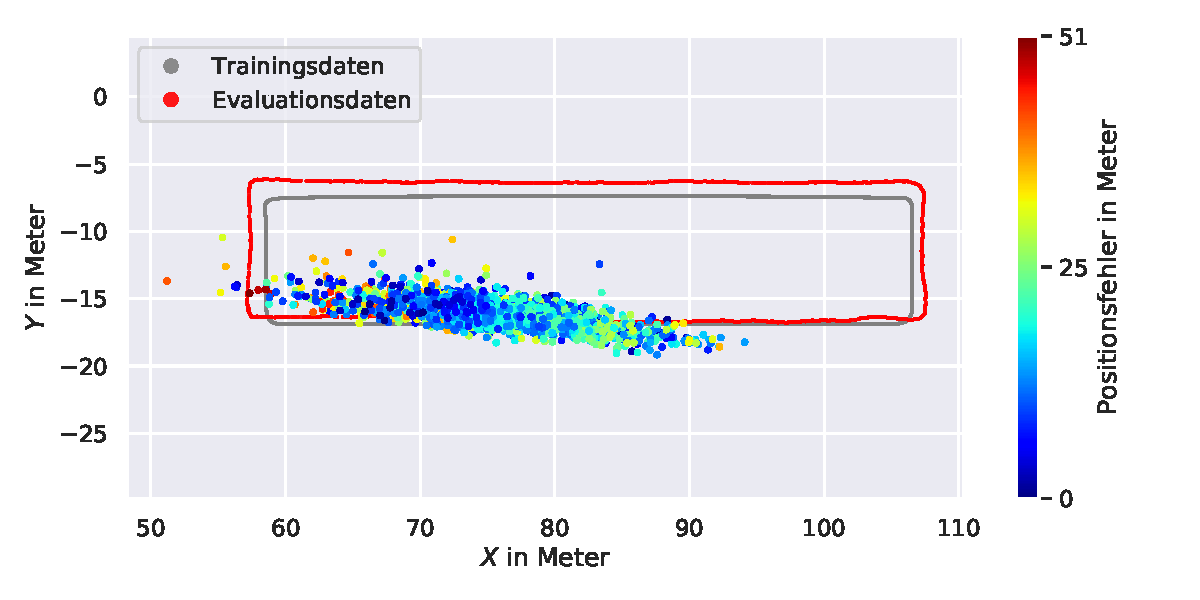
\includegraphics[width=1.0\linewidth]{images/results/ic_cycl/resultsfig_2.pdf} }\\
		\subcaption{} \label{subfig:ic_fig4} & \imagetop{ 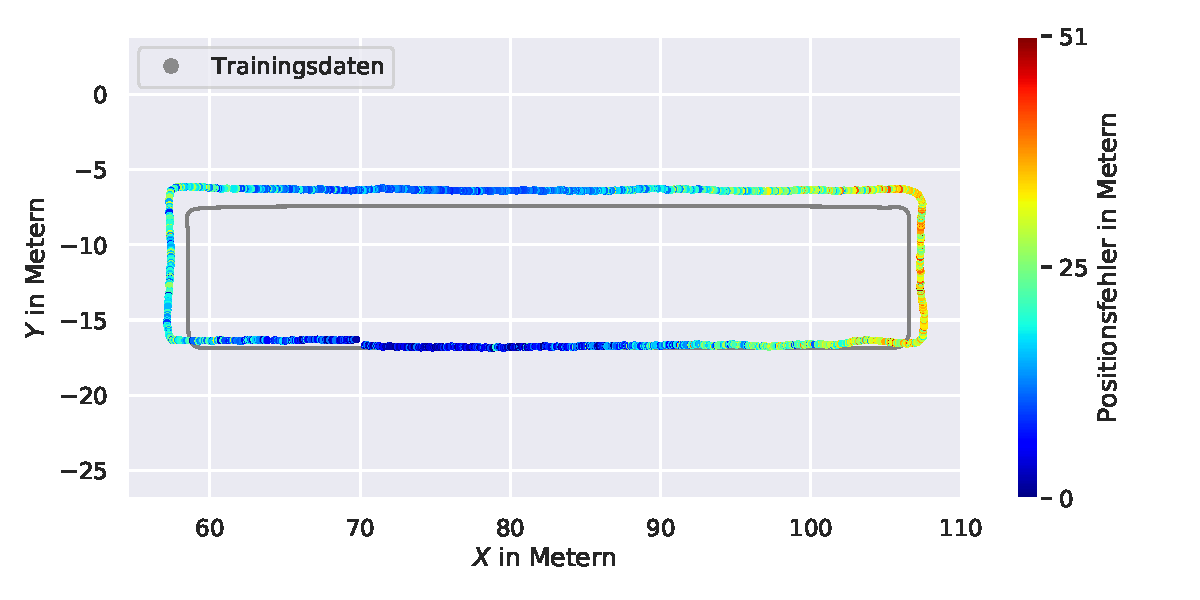
\includegraphics[width=1.0\linewidth]{images/results/ic_cycl/resultsfig_4.pdf} }\\
		\subcaption{} \label{subfig:ic_fig6} & \imagetop{ 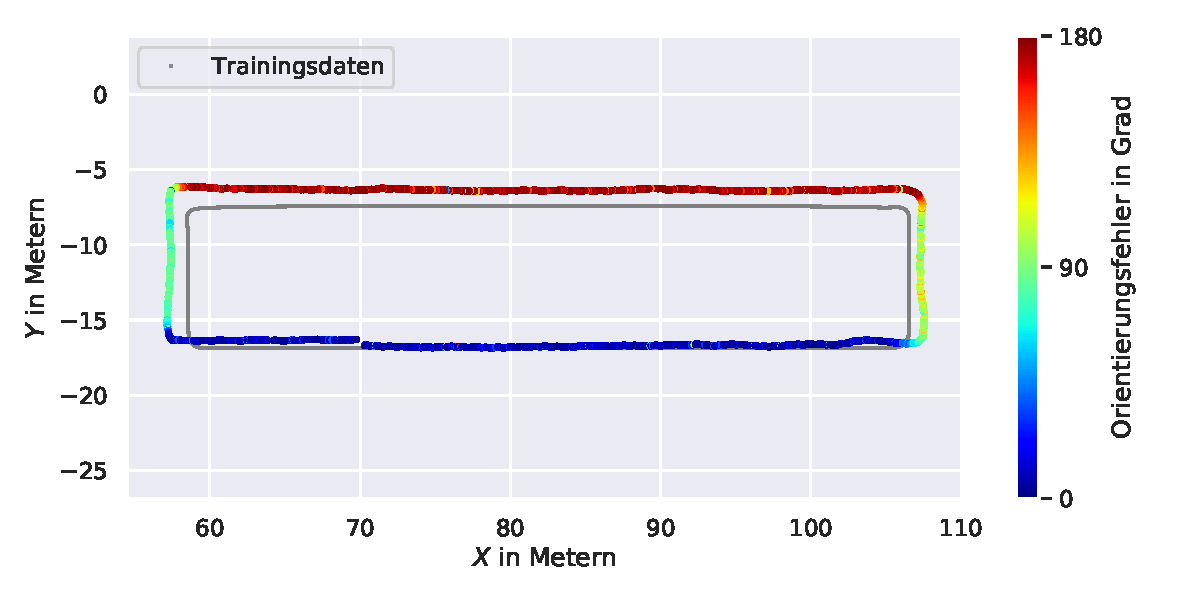
\includegraphics[width=1.0\linewidth]{images/results/ic_cycl/resultsfig_6.pdf} }\\
	\end{tabularx}
	\caption{Visualisierung der Evaluationsergebnisse von der Strecke \textit{IC-loop}. \subref{subfig:ic_fig2} illustriert die Positionen, die von dem KNN bestimmt wurden. \subref{subfig:ic_fig4} stellt die Positionsfehler und \subref{subfig:ic_fig6} die Orientierungsfehler von den jeweiligen Evaluierungsdaten dar. }
	\label{fig:result_ic_loop}
\end{figure}





\begin{table}
	\centering
	\caption{Evaluationsergebnisse von der Strecke \textit{HS-gamma}. Es wird die Akkuratesse der mit den jeweiligen Trainingsdaten trainierten Netzwerke angegeben, die mit den korrespondierenden synthetischen Evaluierungsdaten sowie jeweils mit den realen Evaluationsdaten evaluiert wurden. Mit ausschließlich synthetischen Daten konnte die eine Akkuratesse von 1.00$m$ in der Position und 9.92° in der Orientierung mit den Gradietenbilder der karikaturistischen Simulation erreicht werden. Bei der Evaluierung mit den Gradientenbilder der realen Daten konnte eine Akkuratesse von 8.60$m$ in der Position und 19.59° in der Orientierung auf dem Netzwerk erreicht werden, der mit den Gradietenbilder der karikaturistische Simulation trainiert wurde. Abbildung \ref{fig:result_hs_gamma} visualisiert die Evaluierungsergebnisse von diesem künstlichen neuronalen Netzwerk.}
	\begin{tabularx}{1.0\textwidth}{>{\hsize=1.1\hsize \RaggedRight}X >{\hsize=0.95\hsize \RaggedRight}X >{\hsize=0.95\hsize \RaggedRight}X}
	\textbf{Trainingsdatensatz} \hspace{2cm} (Gradientenbild) & \textbf{synthetische Daten} \hspace{2cm} (Position, Orientierung) & \textbf{reale Daten} \hspace{2cm} (Position, Orientierung)\\
	\hline
		karikaturistische Simulation & 1.00$m$, 9.92° & 8.60$m$, 19.59°\\
		\hline
		synthetisches Kantenbild & 1.07$m$, 8.69° & 10.15$m$, 35.11°\\
		\hline
		fotorealistische Simulation & 1.45$m$, 9.17° & 10.27$m$, 41.60°\\
	\end{tabularx}
	\label{tab:results_hs_gamma}
\end{table}

\begin{figure}
	\setlength\extrarowheight{-15pt}
	\centering
	\begin{tabularx}{1.0\textwidth}{>{\centering\arraybackslash}p{0.05\textwidth} X}
		\subcaption{} \label{subfig:hs_gamma_fig2} & \imagetop{ 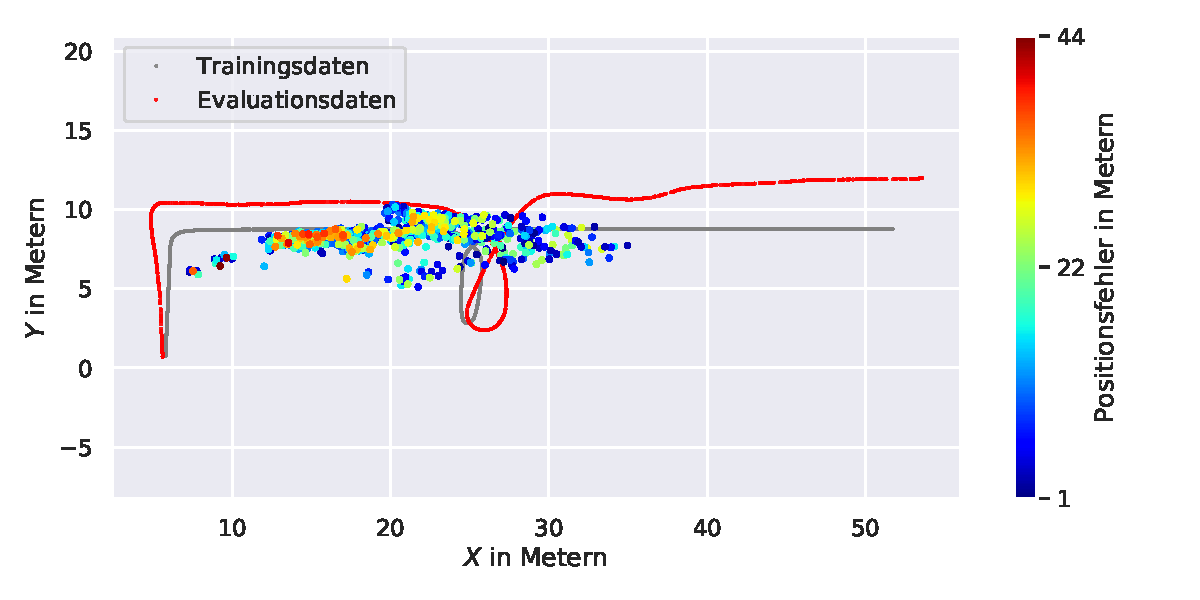
\includegraphics[width=1.0\linewidth]{images/results/hs_gamma/resultsfig_2.pdf} }\\
		\subcaption{} \label{subfig:hs_gamma_fig4} & \imagetop{ 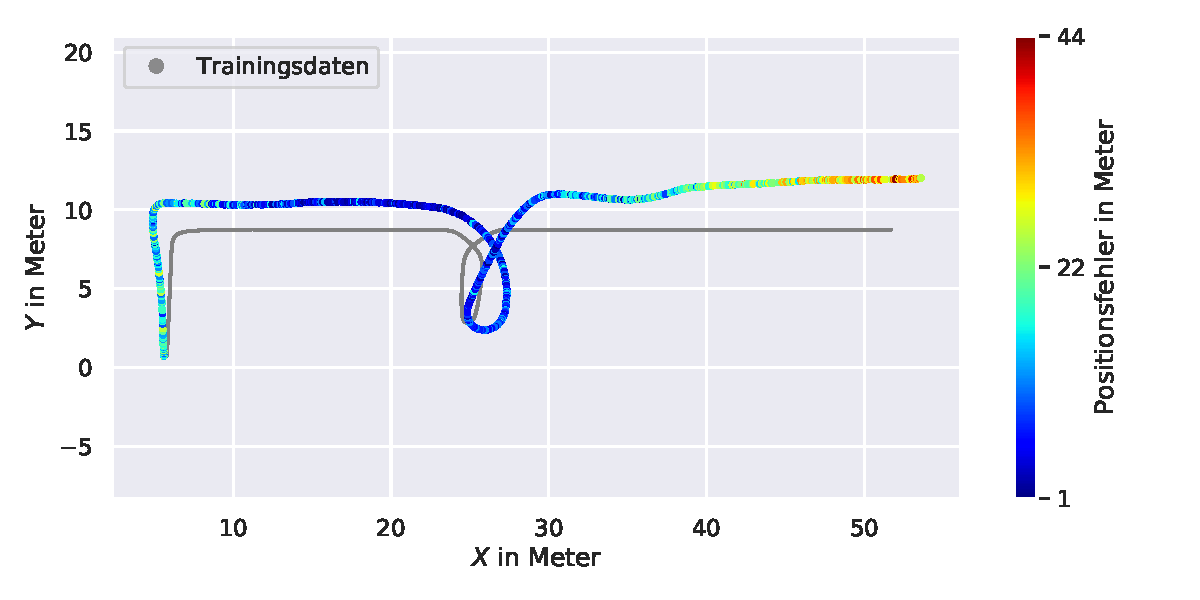
\includegraphics[width=1.0\linewidth]{images/results/hs_gamma/resultsfig_4.pdf} }\\
		\subcaption{} \label{subfig:hs_gamma_fig6} & \imagetop{ 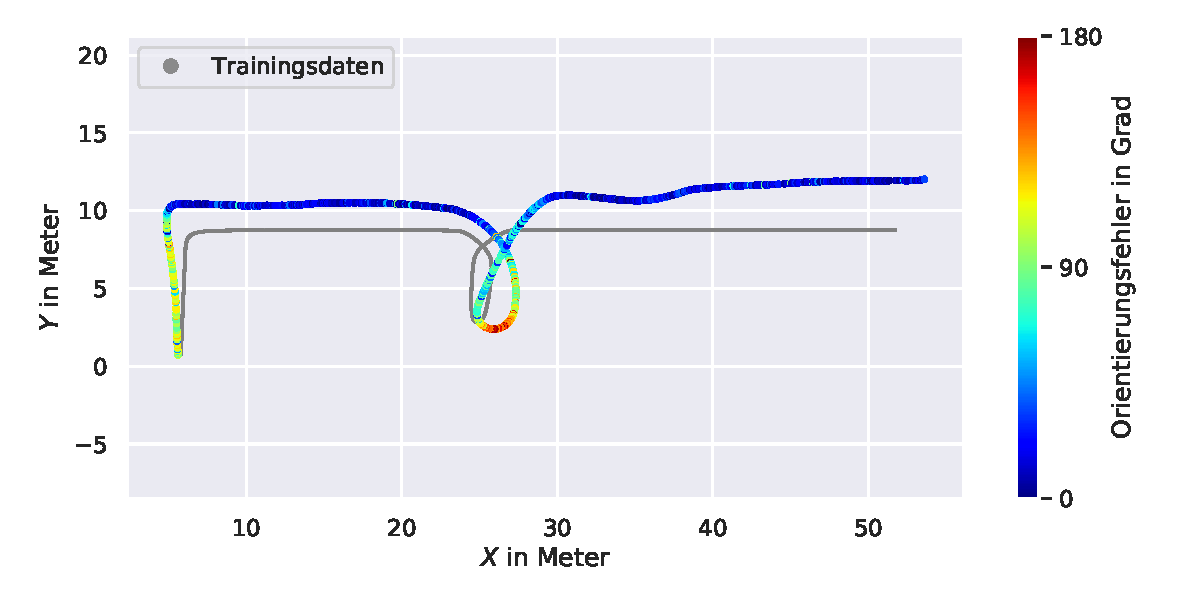
\includegraphics[width=1.0\linewidth]{images/results/hs_gamma/resultsfig_6.pdf} }\\
	\end{tabularx}
	\caption{\subref{subfig:hs_gamma_fig6} HS-gamma}
	\label{fig:result_hs_gamma}
\end{figure}



\begin{table}
	\centering
	\caption{Evaluationsergebnisse von der Strecke \textit{HS-gamma}. Es wird die Akkuratesse der mit den jeweiligen Trainingsdaten trainierten Netzwerke angegeben, die mit den korrespondierenden synthetischen Evaluierungsdaten sowie jeweils mit den realen Evaluationsdaten evaluiert wurden. Mit ausschließlich synthetischen Daten konnte die eine Akkuratesse von 0.82$m$ in der Position und 7.76° in der Orientierung mit den Gradietenbilder der karikaturistischen Simulation erreicht werden. Bei der Evaluierung mit den Gradientenbilder der realen Daten konnte eine Akkuratesse von 4.33$m$ in der Position und 51.64° in der Orientierung auf dem Netzwerk erreicht werden, der mit den Gradietenbilder der synthetischen Kantenbildern trainiert wurde. Abbildung \ref{fig:result_stairs_up} visualisiert die Evaluierungsergebnisse von diesem künstlichen neuronalen Netzwerk.}
	\begin{tabularx}{1.0\textwidth}{>{\hsize=1.1\hsize \RaggedRight}X >{\hsize=0.95\hsize \RaggedRight}X >{\hsize=0.95\hsize \RaggedRight}X}
		\textbf{Trainingsdatensatz} \hspace{2cm} (Gradientenbild) & \textbf{synthetische Daten} \hspace{2cm} (Position, Orientierung) & \textbf{reale Daten} \hspace{2cm} (Position, Orientierung)\\
		\hline
		karikaturistische Simulation & 0.82$m$, 7.76° & 4.77$m$, 23.43°\\
		\hline
		synthetisches Kantenbild & 0.82$m$, 8.48° & 4.33$m$, 51.64°\\
		\hline
		fotorealistische Simulation & 0.92$m$, 7.98° & 5.16$m$, 93.38°\\
	\end{tabularx}
	\label{tab:results_hs_stairs_up}
\end{table}


\begin{figure}
	\setlength\extrarowheight{-15pt}
	\centering
	\begin{tabularx}{1.0\textwidth}{>{\centering\arraybackslash}p{0.05\textwidth} X}
		\subcaption{} \label{subfig:hs_up_fig3} & \imagetop{ 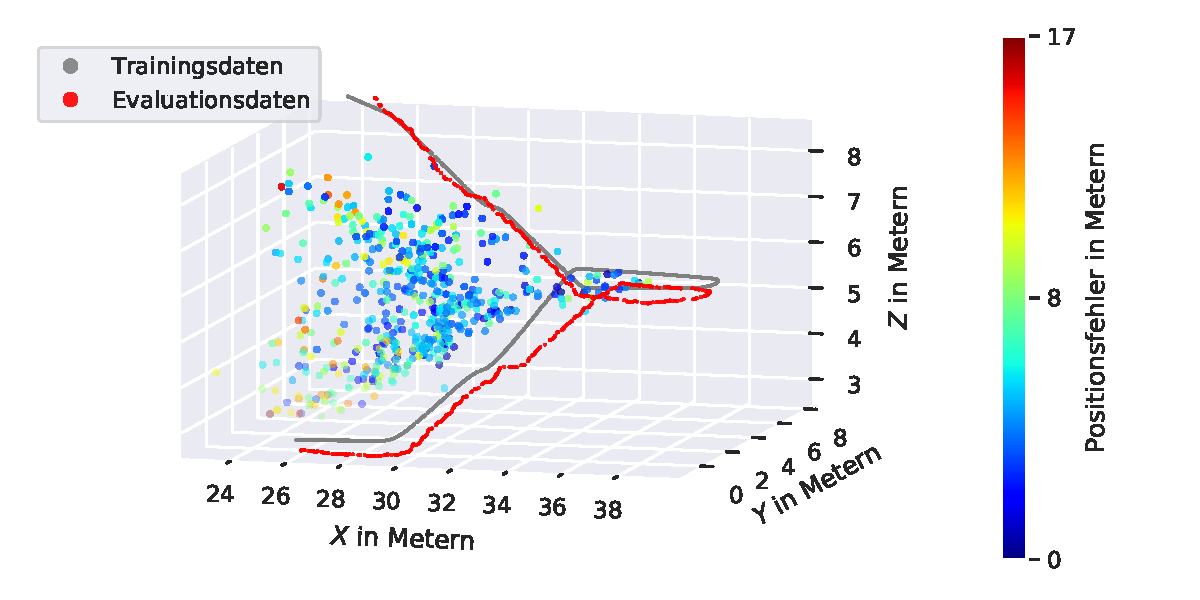
\includegraphics[width=1.0\linewidth]{images/results/hs_up/resultsfig_3.pdf} }\\
		\subcaption{} \label{subfig:hs_up_fig5} & \imagetop{ 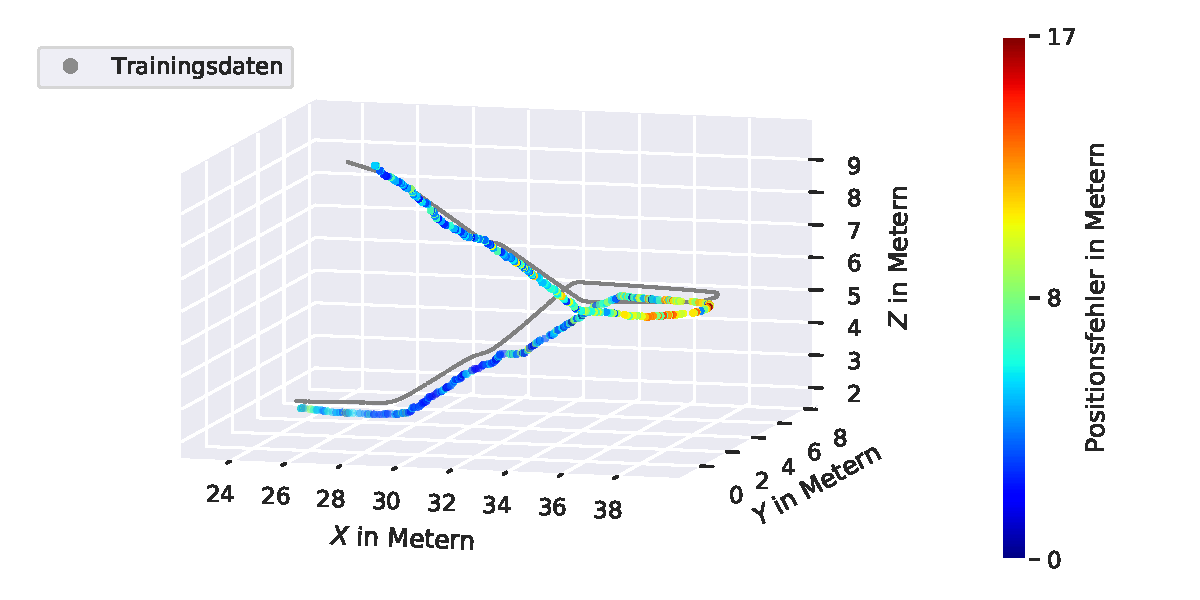
\includegraphics[width=1.0\linewidth]{images/results/hs_up/resultsfig_5.pdf} }\\
		\subcaption{} \label{subfig:hs_up_fig7} & \imagetop{ 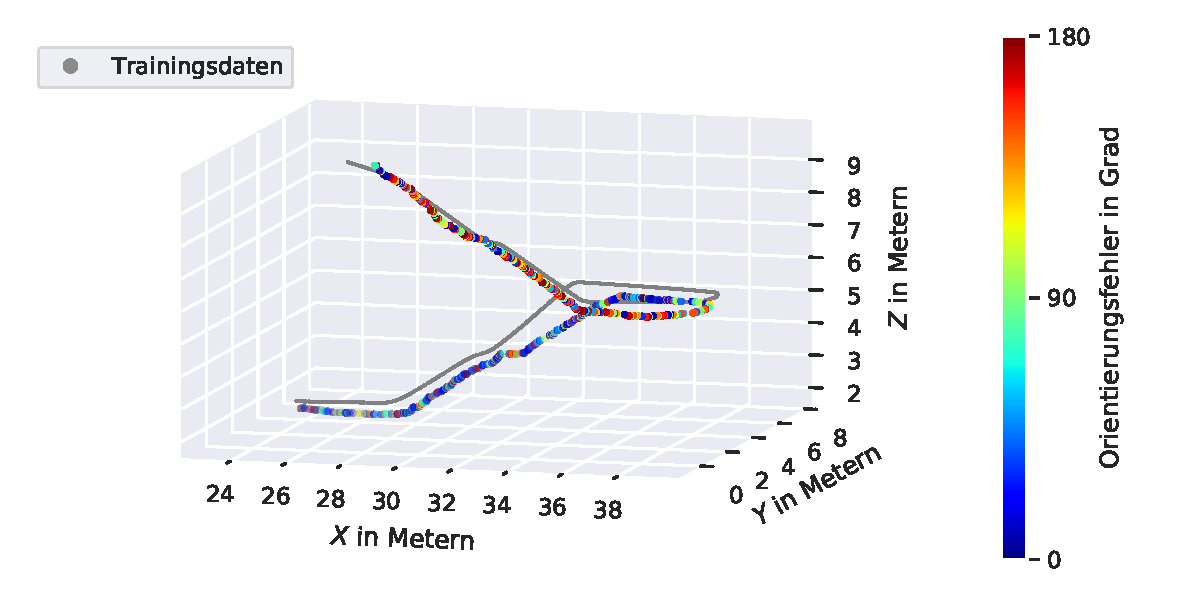
\includegraphics[width=1.0\linewidth]{images/results/hs_up/resultsfig_7.pdf} }\\
	\end{tabularx}
	\caption{\subref{subfig:hs_up_fig7} HS-stairs-up}
	\label{fig:result_hs_stairs_up}
\end{figure}


\begin{table}
	\centering
	\caption{Evaluationsergebnisse von der Strecke \textit{HS-gamma}. Es wird die Akkuratesse der mit den jeweiligen Trainingsdaten trainierten Netzwerke angegeben, die mit den korrespondierenden synthetischen Evaluierungsdaten sowie jeweils mit den realen Evaluationsdaten evaluiert wurden. Mit ausschließlich synthetischen Daten konnte die eine Akkuratesse von 0.85$m$ in der Position und 7.50° in der Orientierung mit den Gradietenbilder der synthetischen Kantenbildern erreicht werden. Bei der Evaluierung mit den Gradientenbilder der realen Daten konnte eine Akkuratesse von 4.20$m$ in der Position und 47.83° in der Orientierung auf dem Netzwerk erreicht werden, der mit den Gradietenbilder der karikaturistische Simulation trainiert wurde. Abbildung \ref{fig:result_stairs_down} visualisiert die Evaluierungsergebnisse von diesem künstlichen neuronalen Netzwerk.}
	\begin{tabularx}{1.0\textwidth}{>{\hsize=1.1\hsize \RaggedRight}X >{\hsize=0.95\hsize \RaggedRight}X >{\hsize=0.95\hsize \RaggedRight}X}
		\textbf{Trainingsdatensatz} \hspace{2cm} (Gradientenbild) & \textbf{synthetische Daten} \hspace{2cm} (Position, Orientierung) & \textbf{reale Daten} \hspace{2cm} (Position, Orientierung)\\
		\hline
		karikaturistische Simulation & 0.91$m$, 8.01° & 4.20$m$, 47.83°\\
		\hline
		synthetisches Kantenbild & 0.85$m$, 7.50° & 5.59$m$, 67.34°\\
		\hline
		fotorealistische Simulation & 1.02$m$, 8.57° & 5.25$m$, 32.70°\\
	\end{tabularx}
	\label{tab:results_hs_stairs_down}
\end{table}


\begin{figure}
	\setlength\extrarowheight{-15pt}
	\centering
	\begin{tabularx}{1.0\textwidth}{>{\centering\arraybackslash}p{0.05\textwidth} X}
		\subcaption{} \label{subfig:hs_down_fig3} & \imagetop{ 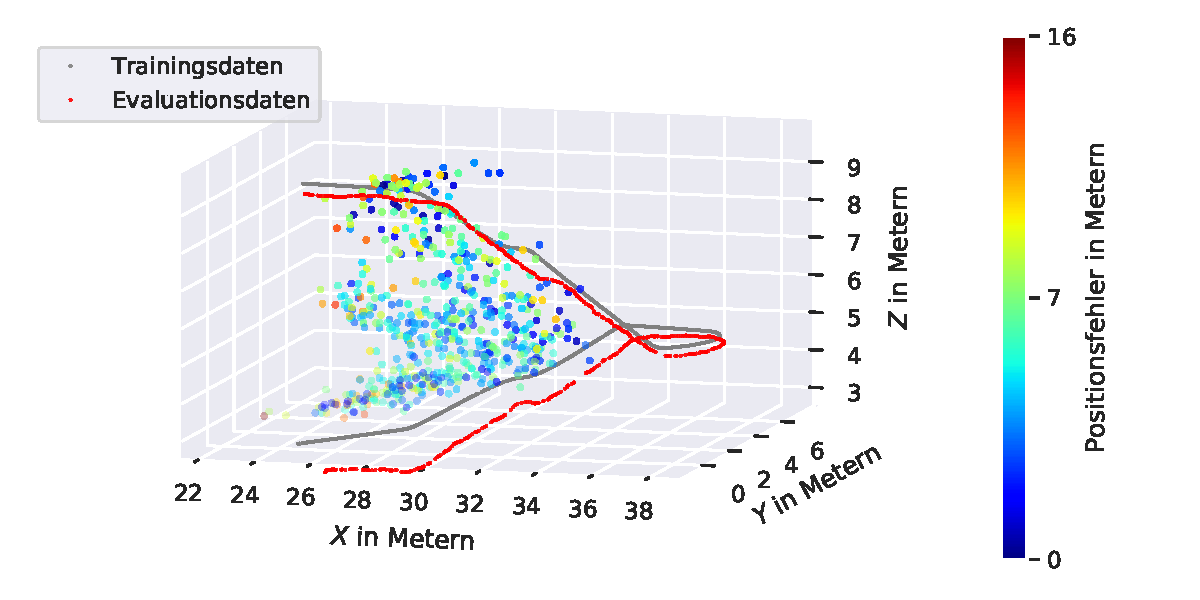
\includegraphics[width=1.0\linewidth]{images/results/hs_down/resultsfig_3.pdf} }\\
		\subcaption{} \label{subfig:hs_down_fig5} & \imagetop{ 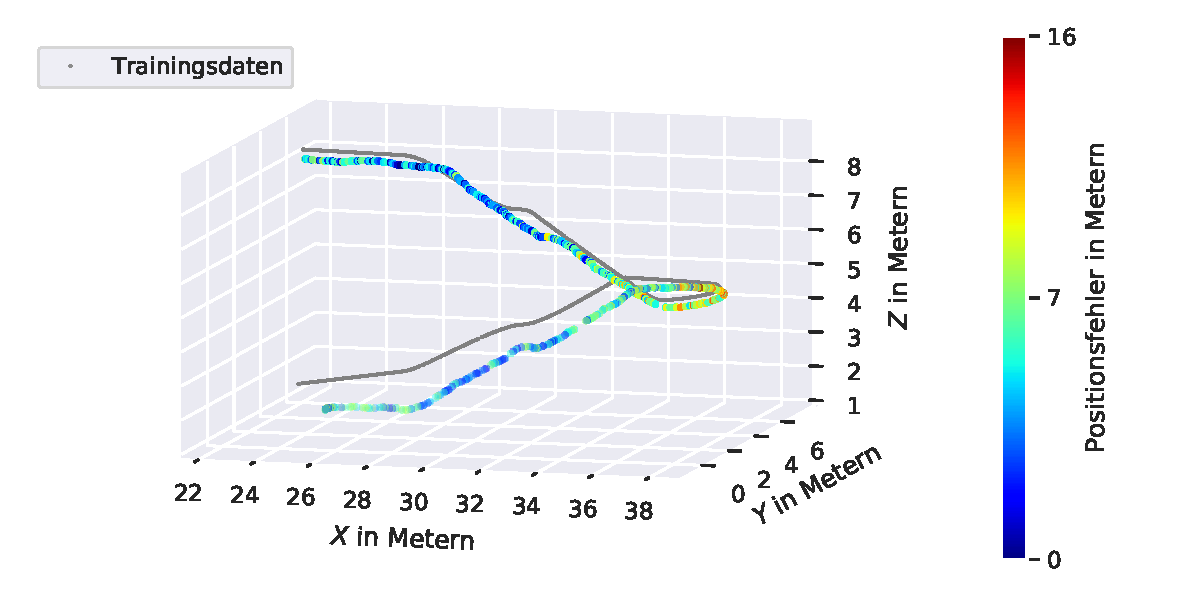
\includegraphics[width=1.0\linewidth]{images/results/hs_down/resultsfig_5.pdf} }\\
		\subcaption{} \label{subfig:hs_down_fig7} & \imagetop{ 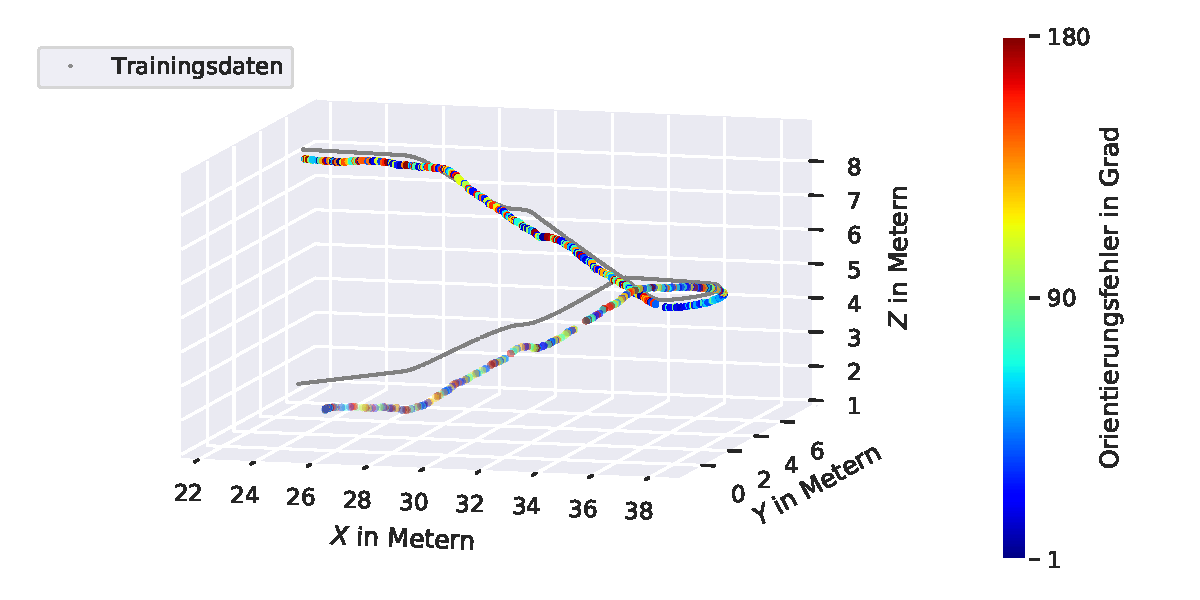
\includegraphics[width=1.0\linewidth]{images/results/hs_down/resultsfig_7.pdf} }\\
	\end{tabularx}
	\caption{\subref{subfig:hs_down_fig7} HS-stairs-down}
	\label{fig:result_hs_stairs_down}
\end{figure}





